%&"../net"
% Reference:
% https://shimowendang.com/docs/wGQPHvHrcTTDyChh/read
\endofdump
\tikzexternalize[prefix=cache/]{lab03}
\begin{document}
\title{Socket Programming}
\maketitle
\tableofcontents

\vfill
You will implement a simple file share application using TCP Socket APIs. 

You can use any programming language. You need to submit your code together with a report. The report should contain how to run your program and some evaluation results.
\vfill
\clearpage
\section{C/S 模型}

\subsection{C/S 模型要求}

\begin{enumerate}
    \item Implement C/S model: 
    \begin{enumerate}
        \item Server listens to a given port (>1024, e.g. 2680)
        \item Multiple clients request the same file from the server
        \item Each client save the file to its local directory.
    \end{enumerate}
    \item Use Mininet to compare the overall file downloading time. Study how the number of downloading time changes with respect to the number of peers. You need to create the following star topology in Mininet. You can use one host as a server, and the other hosts as peers requesting files.
    \begin{figure}[H]
        \centering
        \begin{tikzpicture}[font=\Large]
\node (s) at (0,0) {\faServer};
\node (c1) at (0,2) {\faLaptop};
\node (c2) at (2,1) {\faLaptop};
\node (c3) at (2,-1) {\faLaptop};
\node (c4) at (0,-2) {\faLaptop};
\node (c5) at (-2,-1) {\faLaptop};
\node (c6) at (-2,1) {\faLaptop};
\draw  (c1) edge (s);
\draw  (c2) edge (s);
\draw  (c3) edge (s);
\draw  (c4) edge (s);
\draw  (c5) edge (s);
\draw  (c6) edge (s);
\end{tikzpicture}
    \end{figure}
\end{enumerate}

\subsection{C/S 模型测试}

在 root 模式下,使用 \verb"csmodel" 文件夹下的 \verb"cspy_test.sh" 脚本即可测试。

\begin{figure}[H]
    \centering
    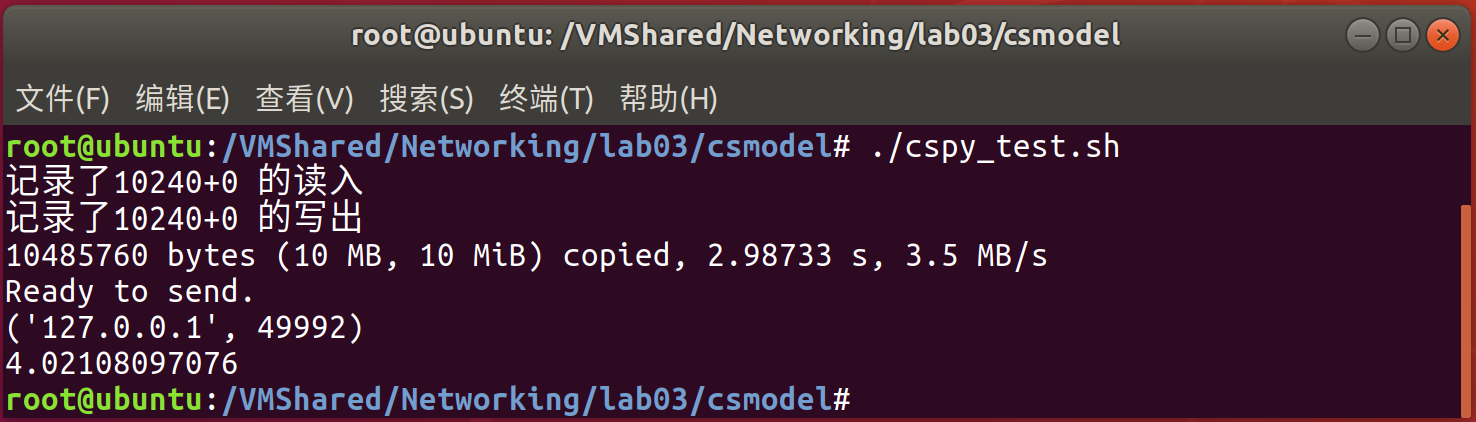
\includegraphics[width=\linewidth]{cspytest}
    \caption{单机测试}
\end{figure}

本地测试将会在服务器与客户端之间,在 \verb"2683" 端口上传输 10 MB 的文件,传输时长大概在 4s 左右。如果最后没有比较上的异常,就说明被完整地传输了。

\code[language=bash]{csmodel/cspy\_test.sh}

而对于 Mininet 模拟来说,使用 \verb"python" 运行 \verb"csmodel/centralized.py" 脚本即可开始测试星状结构的网络。运行脚本后需要输入测试的主机数量。如果脚本后面添加参数 \verb" py --dirty" 则可以跳过一些检查,这对于客户机数量多的情况比较有用。

\begin{figure}[H]
    \centering
    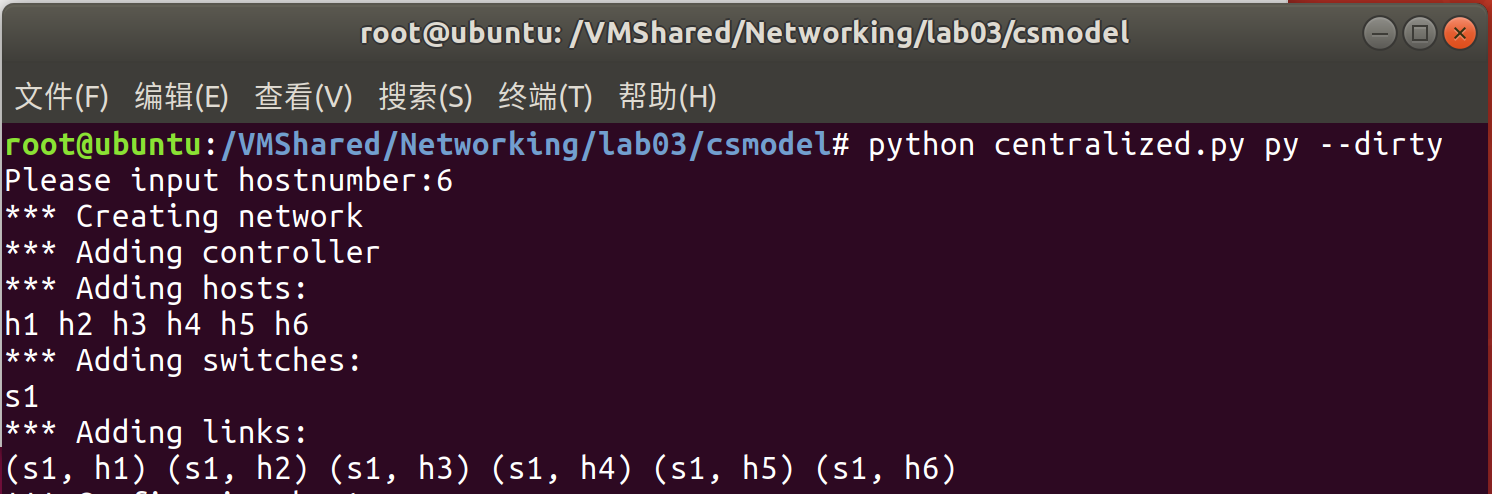
\includegraphics[width=0.6\linewidth]{runcsmodel}
    \caption{C/S Mininet 测试}\label{fig:csmodelrun}
\end{figure}

由图 \ref{fig:csmodeltest} 所示,所有的客户机会同时从服务器获取上述的 10MB 文件,每个客户机会在完成传输后各自存储为对应的 \verb"file_receive_h*.txt" 文件,并将计时结果写入文件 \verb"result_py.dat",当 Mininet 退出 CLI 的时候(\verb"quit"指令),就会对结果进行统计,并给出平均时间。

\begin{figure}[H]
    \centering
    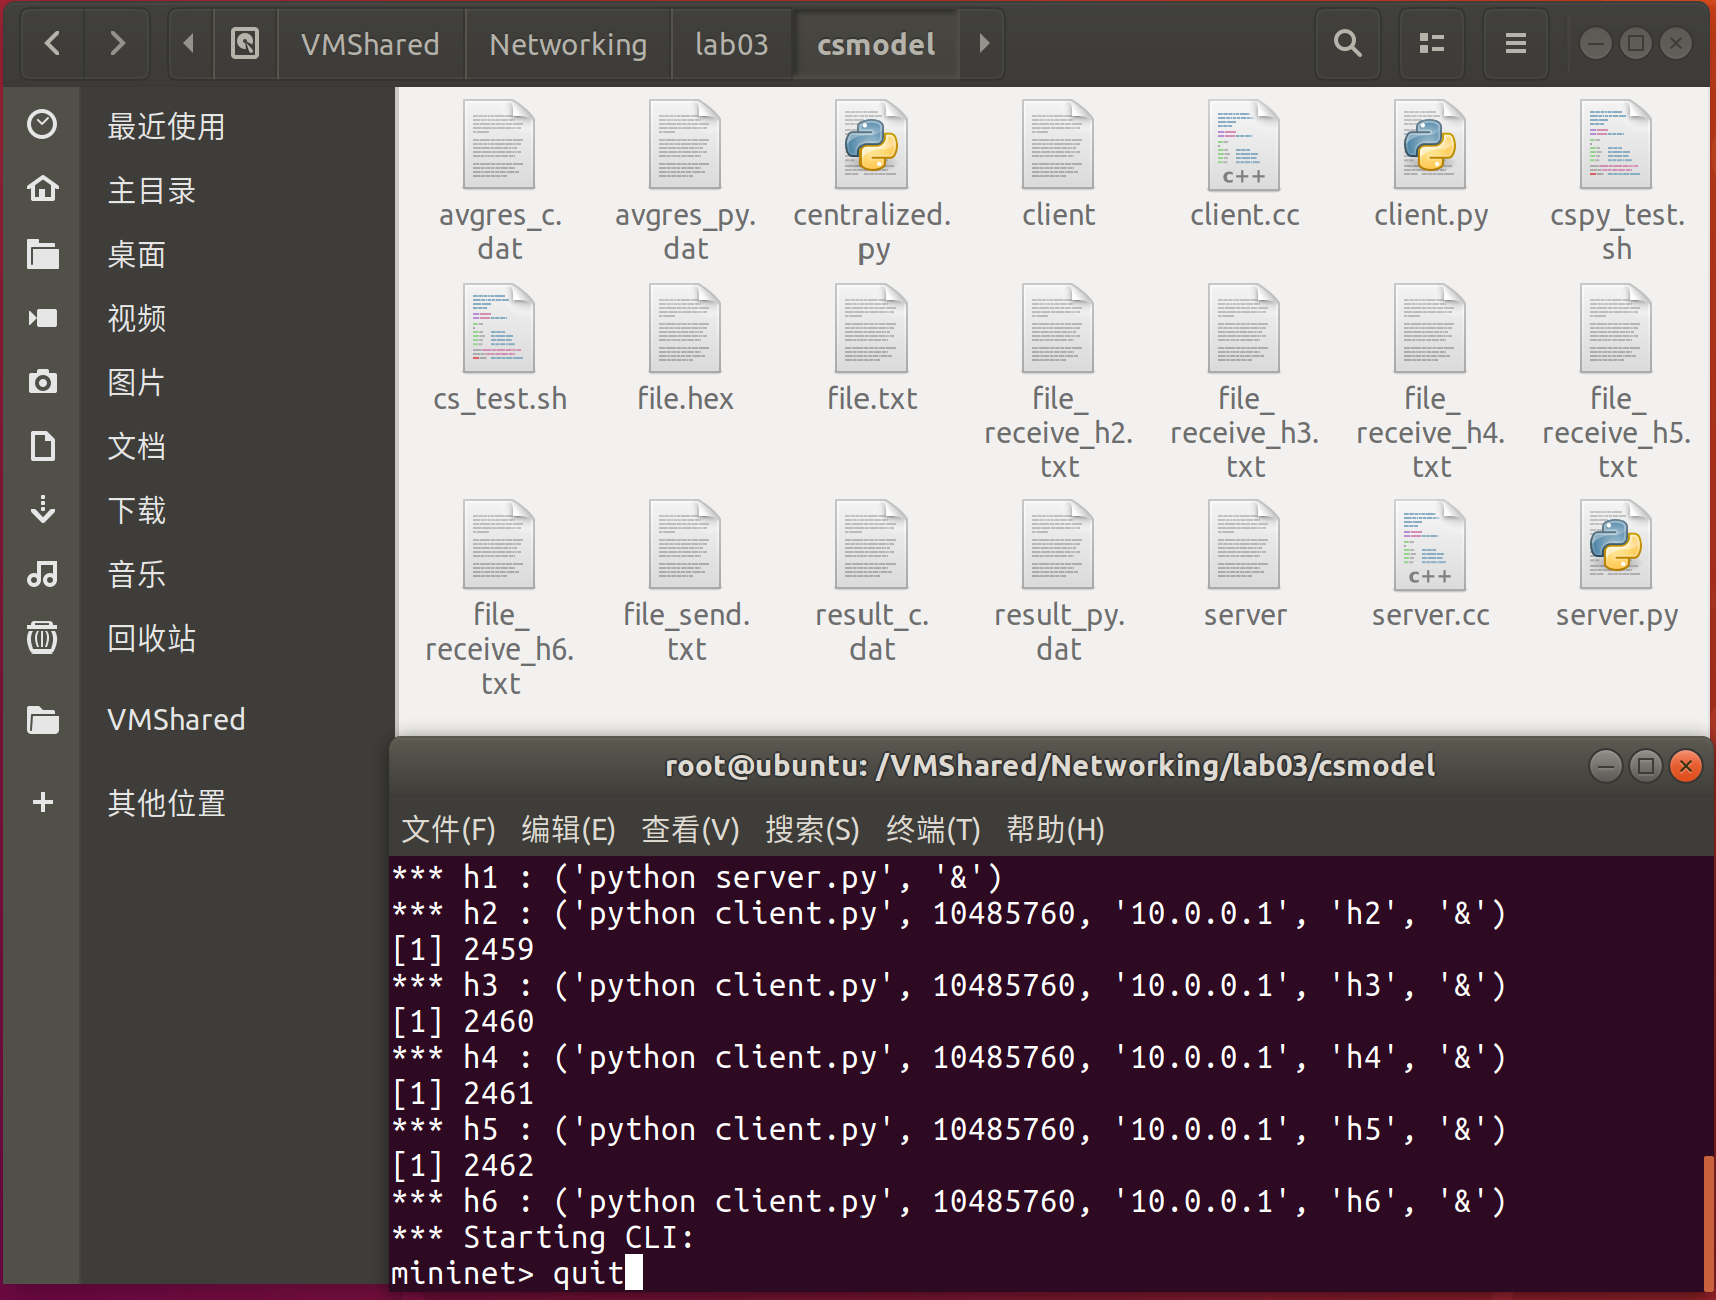
\includegraphics[width=0.5\linewidth]{centralized}
    \caption{运行多机测试}\label{fig:csmodeltest}
\end{figure}

由图 \ref{fig:csmodelstat} 可见,随着客户机的增长,传输时间也会显著变长。

\begin{figure}[H]
    \centering
    \begin{tikzpicture}
        \begin{axis}[xmin={0},
        ymin={0},
        xlabel={\# Client},
        ylabel={Avg Transfer Time (s)},
        grid={major},
        ]
         \addplot+ [] table[] {csmodel/avgres_py.dat};
        \end{axis}
    \end{tikzpicture}
    \caption{不同的客户机数量下平均传输时间}\label{fig:csmodelstat}
\end{figure}    

\section{P2P 模型}

\subsection{P2P 模型要求}

\begin{enumerate}
    \item Implement P2P model: Each peer downloads part of the file from the server, and then distributes it to all the other peers.

    \item Use Mininet to compare the overall file downloading time under P2P model.
    
    \item For peer-to-peer mode, you may want to design a tracker file first. The tracker file contains the following information:
    
    \begin{table}[H]
    \centering
    \begin{tabular}{ll}
        \toprule
        file chunk id & peer ip \\
        \midrule
        1 & 10.0.0.1\\
        2 & 10.0.0.2\\
        3 & 10.0.0.3\\
        4 & 10.0.0.4\\
        \bottomrule
    \end{tabular}
    \end{table}

    Then, if a client wants piece 2, it will contact 10.0.0.2. If the peer with ip=10.0.0.2 does not have the piece yet, it will contact the server to download this piece first. 
\end{enumerate}

\subsection{P2P 模型测试}

使用 \verb"p2pmodel/p2ptest.sh" 可以进行批量测试,这一步可以创建一个 10MB 大小的文件 \verb"file.txt"。当然也可以直接运行 \verb"python" 脚本进行测试:
\begin{verbatim}
    sudo python p2pmodel/centralized.py 5
\end{verbatim}
最后一个参数用于指定主机数量。

\begin{figure}[H]
    \centering
    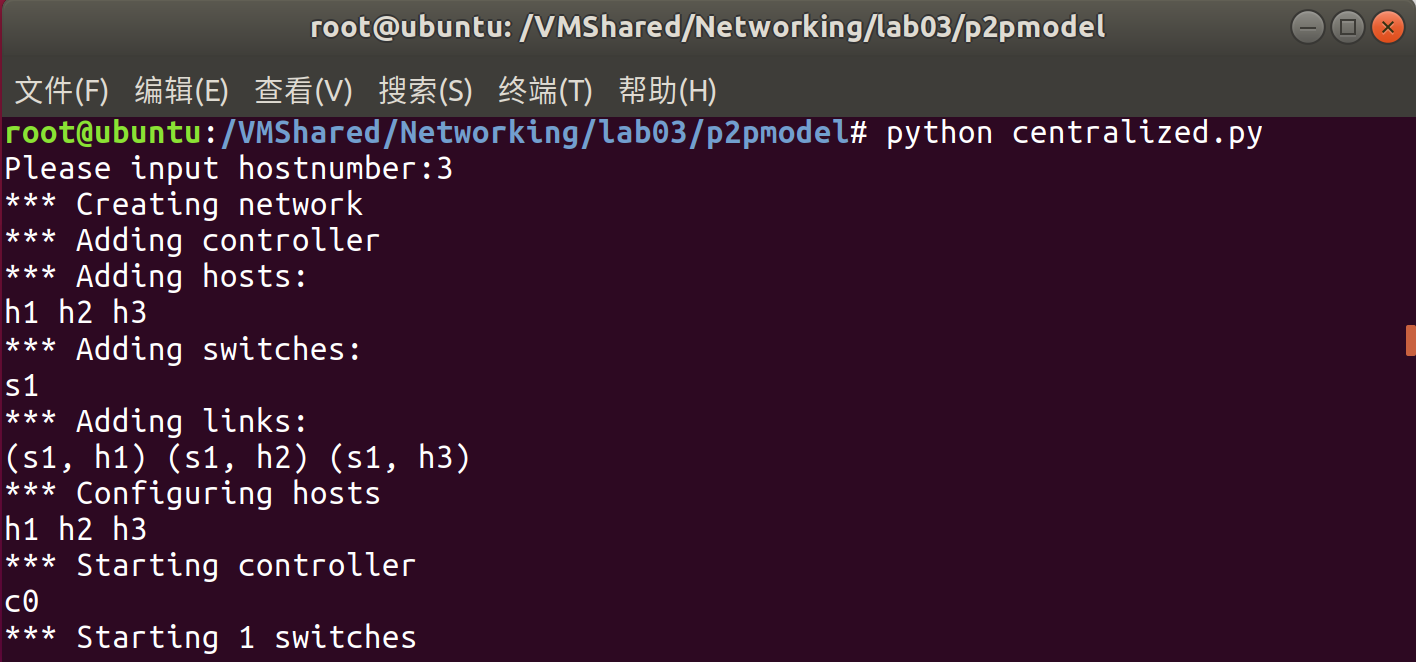
\includegraphics[width=0.6\linewidth]{runp2pmodel}
    \caption{P2P Mininet 测试}\label{fig:p2pmodelrun}
\end{figure}

\code[language=bash]{p2pmodel/p2ptest.sh}

\begin{figure}[H]
    \centering
    \begin{tikzpicture}
        \begin{axis}[xmin={0},
        ymin={0},
        xlabel={\# Peer},
        ylabel={Avg Transfer Time (s)},
        grid={major},
        ]
         \addplot+ [] table[] {p2pmodel/avgres_py.dat};
        \end{axis}
    \end{tikzpicture}
    \caption{不同的对等方数量下平均传输时间}\label{fig:p2pmodelstat}
\end{figure}

\appendix

\section{C/S 模型架构实现}

下面给出了 Mininet 配置的具体代码。实际上星状网络可以采用 \verb"LinearTopo" 代替,此处为了更好地控制源码,就采用了手写的 \verb"CentralizedTopo" 网络结构。

\code{csmodel/centralized.py}

\section{C/S 模型 Python 实现 \faPython}

为了方便理解 TCP 网络模型,先跟着书用 Python 实现了一遍多线程 C/S 模型。

下面是服务器端的代码,在主循环中由 \verb"accept()" 阻塞接收,一旦有客户机进入就会开辟新的线程进行文件传输。

\code{csmodel/server.py}

下面是客户端代码,由于 TCP 连接接收大小有一定的限制,超过限制可能就会产生长期接收不到的情况,所以每次只会接收 1024 字节,分为多次进行接收。由于 Python 内存访问比较慢,这里直接就写入了文件,没有首先将内容进入内存。

\code{csmodel/client.py}

\section{C/S 模型 C 实现 \textsf{C}}

如果想运行 C 语言版本,进行单机测试:
\begin{figure}[H]
    \centering
    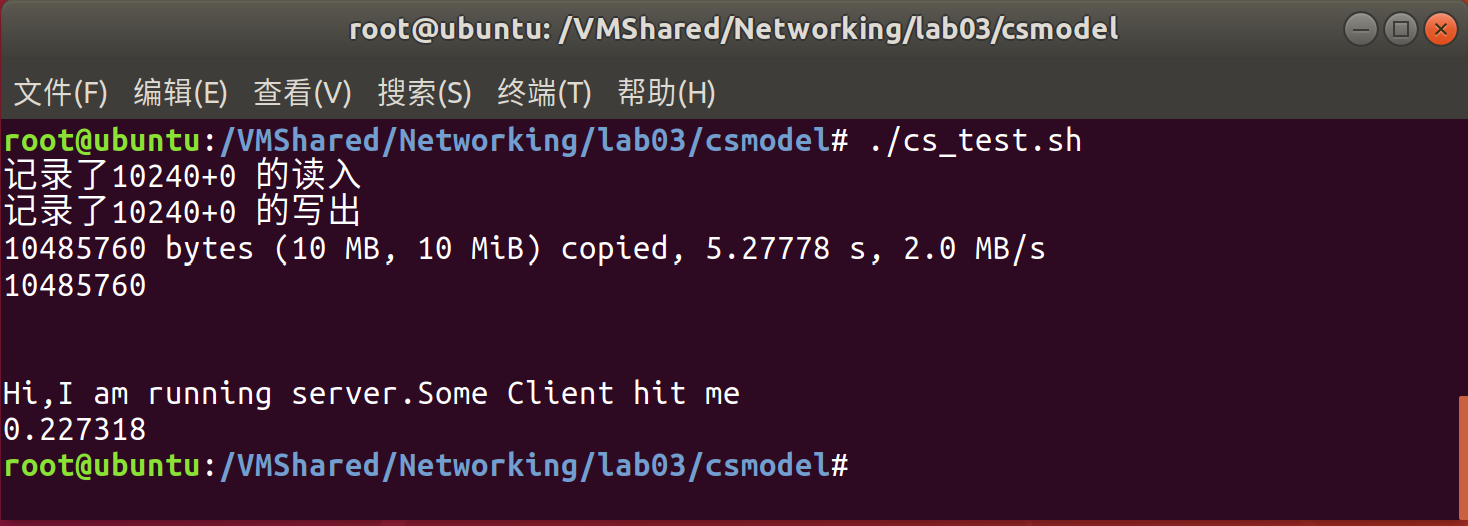
\includegraphics[width=0.7\textwidth]{cstest}
    \caption{C 语言单机测试}
\end{figure}

进行 Mininet 测试需要使用参数 \verb" c --dirty"。

\begin{figure}[H]
    \centering
    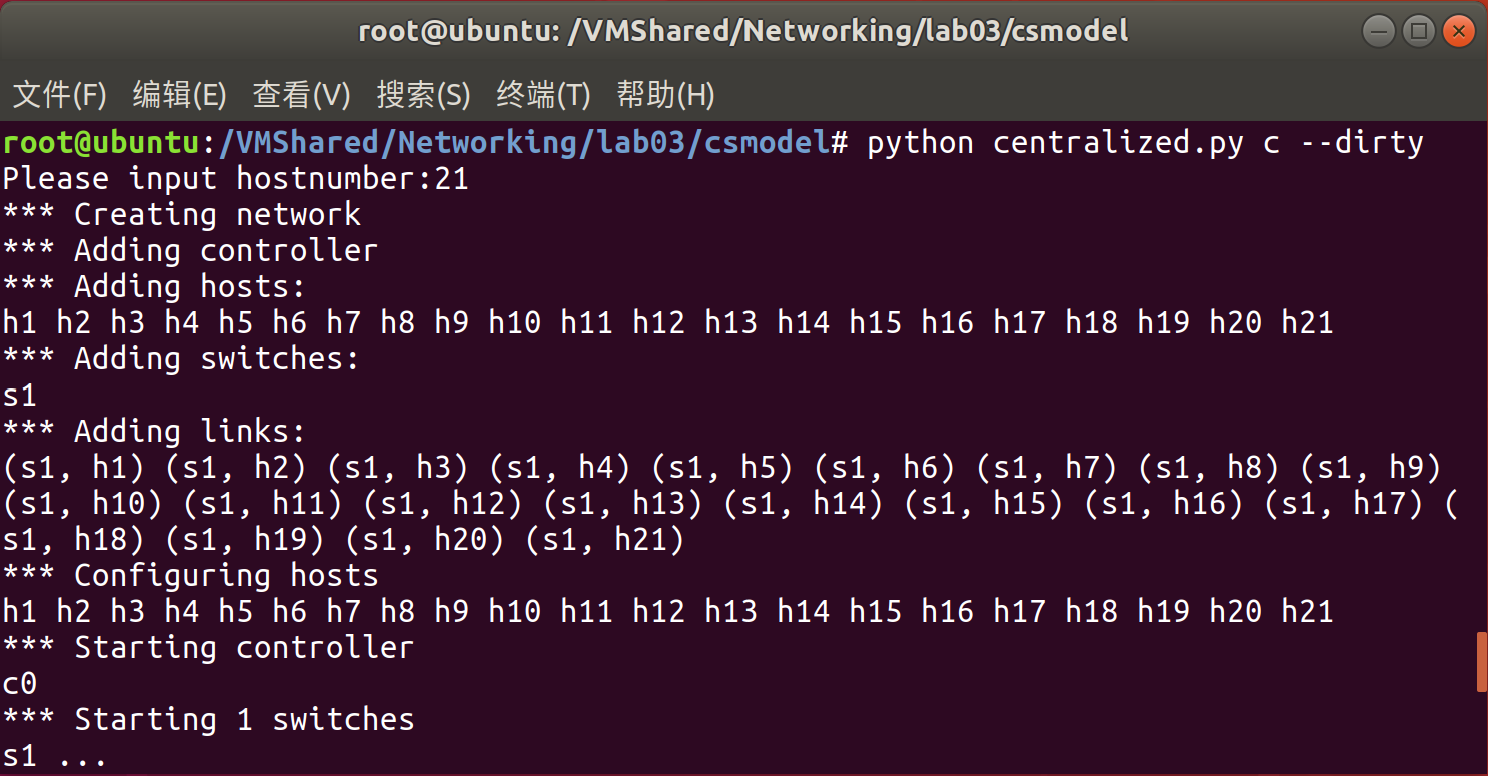
\includegraphics[width=0.6\textwidth]{cruncsmodel}
    \caption{C 语言多机测试}
\end{figure}

可见使用 C 语言效率更高,1s 不到就可以完成,这也导致如果需要对其评测需要使用很大的文件,否则数据差距并不明显,这里就跳过对 C 语言实现版本的测评部分。下面的代码主要是对示例代码的一些改进而得到的。

\code[language=c]{csmodel/server.cc}

\code[language=c]{csmodel/client.cc}

\section{P2P 模型架构实现}

\code{p2pmodel/centralized.py}

\section{P2P 模型 Python 实现 \faPython}

服务器与 C/S 模型的差距不大,主要可以接收一个文件块的参数。

\code{p2pmodel/server.py}

对等方的实现相对复杂。

\code{p2pmodel/peer.py}

\end{document}